% ============================================================
%  CONCEPTOS CLAVE
%  - Todo lo que empieza con % es un COMENTARIO (no se imprime)
%  - Los COMANDOS empiezan con \ (backslash)
%  - Los ENTORNOS se abren con \begin{...} y se cierran con \end{...}
%  - Las LLAVES { } agrupan argumentos obligatorios
%  - Los CORCHETES [ ] agrupan argumentos opcionales
% ============================================================

% 1. CLASE DEL DOCUMENTO
%    Define el tipo general: article, report, book, etc.
%    [12pt]       → tamaño de fuente base
%    [a4paper]    → tamaño de hoja
\documentclass[12pt, a4paper]{article}

% ── PAQUETES ─────────────────────────────────────────────────
% Los paquetes amplían las capacidades de LaTeX.
% Se cargan en el "preámbulo" (antes de \begin{document}).

\usepackage[utf8]{inputenc}       % Permite tildes y ñ
\usepackage[spanish]{babel}       % Idioma español (guiones, fechas, etc.)
\usepackage{geometry}             % Control de márgenes
\usepackage{graphicx}             % Para insertar imágenes
\usepackage{setspace}             % Control de interlineado
\usepackage{hyperref}             % Links clicables (índice, URLs)
\usepackage{xcolor}               % Colores personalizados
\usepackage{listings}
\usepackage{tcolorbox}
\usepackage{amsmath}
\usepackage{float}
\usepackage{booktabs}
\tcbuselibrary{listings, skins}

\newtcblisting{terminal}{
    colback   = black,           % fondo negro
    colframe  = gray!50,         % borde gris
    coltitle  = white,           % título en blanco
    coltext   = green!70!white,  % texto verde (estilo terminal clásica)
    title     = Terminal,
    fonttitle = \bfseries\small,
    listing only,
    listing options = {
        basicstyle = \ttfamily\small\color{green!70!white},
        breaklines = true,
    }
}

\lstset{
    basicstyle    = \ttfamily\small,   % fuente monoespaciada
    keywordstyle  = \color{blue},      % palabras clave en azul
    commentstyle  = \color{gray},      % comentarios en gris
    stringstyle   = \color{orange},    % strings en naranja
    numbers       = left,              % números de línea a la izquierda
    frame         = single,            % recuadro alrededor del bloque
    breaklines    = true,              % corta líneas largas automáticamente
}
% ── DATOS DEL DOCUMENTO ──────────────────────────────────────
% Definimos variables reutilizables con \newcommand
\newcommand{\tema}{Trabajo Práctico Nº1: Python}
\newcommand{\titulotrabajo}{Informe}
\newcommand{\autor}{Alfici, Facundo Ezequiel}
\newcommand{\documento}{44012327}
\newcommand{\curso}{PROCOM}
\newcommand{\fundacion}{Fundación Fulgor}
\newcommand{\fecha}{\today}        % \today imprime la fecha actual automáticamente


% ── INICIO DEL DOCUMENTO ─────────────────────────────────────
% Todo lo visible va DENTRO de este entorno
\begin{document}

% Quitamos la numeración en la carátula
\thispagestyle{empty}

% ── CARÁTULA ─────────────────────────────────────────────────
\begin{center}   % Entorno para centrar contenido

    % --- Encabezado institucional ---
    {\Large \textbf{\fundacion}}\\[0.3cm]      % \\ fuerza un salto de línea                 % [0.2cm] = espacio extra después
    {\large \curso}

    \vspace{1.5cm}   % Espacio vertical de 1.5 cm

    % --- Logo (opcional) ---
    % Descomenta las 2 líneas siguientes si tenés un logo guardado
    % \includegraphics[width=0.25\textwidth]{logo.png}
    % \vspace{1cm}

    \hrule height 1pt   % Línea horizontal
    \vspace{0.4cm}

    % --- Título del trabajo ---
    {\LARGE \textbf{\titulotrabajo}}\\[0.3cm]
    {\large \tema}

    \vspace{0.4cm}
    \hrule height 1pt

    \vspace{2.5cm}

    % --- Datos del alumno ---
    % Tabla simple de 2 columnas: etiqueta y valor
    \begin{tabular}{r l}   % r = columna alineada a la derecha, l = izquierda
        \textbf{Autor:}   & \autor\\[0.2cm]
        \textbf{Documento:}  & \documento\\[0.2cm]
        \textbf{Docentes:} &  Ariel Pola, Santiago Garaventta Pascual y Agustín Pesce\\
    \end{tabular}

    \vspace{3cm}

    % --- Fecha ---
    {\large \fecha}

\end{center}

% Salto de página → el informe real comienza en la siguiente hoja
\newpage

% ── EJEMPLO DE PRIMERA SECCIÓN (para no dejar el doc vacío) ──
\tableofcontents   % Genera el índice automáticamente
\newpage

\section{Introducción}
En este laboratorio se buscará realizar un programa en Python que permita utilizar la comunicación serie
para enviar y recibir datos desde el puerto virtual de Windows, con los cuales se generarán y graficarán filtros.

Para ello se utilizará el script \texttt{com\_serie.py}, que se encargará de enviar y recibir los datos desde el puerto.
Estos datos se enviarán hacia el archivo \texttt{main.py}, el cual tiene la tarea de procesar lo recibido y, según el comando,
realizar las distintas acciones propuestas por el enunciado.

También se importó la clase \texttt{RaisedCosineFilter}, que es proveniente del archivo \texttt{filtros.py}. Esta clase se encargará de la generación de los filtros, siendo invocada
desde el script \texttt{main.py} cada vez que se reciba el comando correspondiente.

\section{Desarrollo}
Para comenzar con el desarrollo, se realizará un marco teórico sobre los filtros que se desean generar.
\subsection{Marco Teórico}
Como parte principal del trabajo, se utilizaron filtros Raised Cosine (RC)
y Root Raised Cosine (RRC), los cuales forman parte de los filtros FIR, debido a que necesitan una respuesta al impuslo finita (de N muestras) y una fase lineal.
\subsubsection{Filtros FIR}
    En lo que se refiere a los filtros FIR (Finite Impulse Response), podemos describir su funcionamiento utilizando la siguiente expresión,
    donde tomamos en cuenta coeficientes de realimentación nulos tal que
    ($a_k = 0 \; \forall k$)
    \begin{equation}
        y[n] = \sum_{k=0}^{N} h[k] \, x[n-k]
        \label{eq:fir}
    \end{equation}
    donde se tiene que h[k] es la respuesta al impulso.

    Las propiedades más importantes de este tipo de filtros son:
    \begin{itemize}
        \item \textit{Estabilidad absoluta}
        \item \textit{Fase lineal}
        \item \textit{Independencia de muestras pasadas}
    \end{itemize}
\subsubsection{Filtros RC y RRC}
    El filtro \textit{\textbf{Raised Cosine (RC)}} es la solución canónica al criterio de Nyquist, cuyo ancho de banda podemos manejar en base
    a un parámetro llamado roll-off($\beta$), el cuál responde a la siguiente expresión.
    \begin{equation}
        W_{\text{RC}} = \frac{1 + \beta}{2T}
        \label{eq:wrc}
    \end{equation}
    
    Una de las características más importantes de este filtro es la propiedad de
    \textbf{Interferencia Inter Símbolo (ISI)} nula. Donde, para cada $t=nT$, se tiene una ISI nula.

    Respecto al filtro \textit{\textbf{Root Raised Cosine (RRC)}}, se utiliza para sistemas de comunicaciones reales, específicamente
    en sistemas donde se debe adaptar el transmisor Tx con el receptor Rx, de tal manera que se tiene que:
    \begin{equation}
        \boxed{H_{\text{RRC}}(f)*H_{\text{RRC}}(f) = H_{\text{RC}}(f)}
    \end{equation}
    Pues una de las características más importantes de este filtro es que:
    \begin{equation}
        H_{\text{RRC}}(f) = \sqrt{H_{\text{RC}}(f)}
    \end{equation}
    Donde se puede aprovechar las características mas beneficiosas del filtro \textit{\textbf{RC}} y tener sistemas adaptados al mismo tiempo.
    
    Algo importante a destacar antes de pasar a la siguiente sección, es definir los conceptos de los parámetros que se deberán cargar a los filtros, estos
    parámetros se describen a continuación.
    \begin{itemize}
        \item \texttt{\textbf{alpha}} ---
            Representará el factor de \textbf{roll-off}. Es un float que debe tomar valores entre 0 y 1.
        \item \texttt{\textbf{span}} ---
            Se refiere a la duración total del filtro expresado en cantidad de símbolos. Es decir, sabiendo que la respuesta al impulso se extenderá
            un tiempo determinado, este parámetro representa ese tiempo traducido a símbolos.
        \item \texttt{\textbf{sps}} ---
            También llamado \textbf{Samples Per Symbol}, representa sobre las muestras por símbolo, donde cada símbolo representará a 
            la señal como una forma de onda o como un punto (según si es TD o TC).
            Cuanto mayor sean las SPS, más precisa será la representación de la respuesta al impulso.
    \end{itemize}
\subsection{Comandos}
A continuación, se explicarán los diferentes comandos que se implementaron en el script \texttt{main.py}.
\begin{itemize}
    \item \texttt{generate\_filter:(\textit{alpha}, \textit{span}, \textit{sps}, \textit{rrc})} ---
    Genera un filtro con los parámetros indicados.
        \begin{description}
            \item[\texttt{alpha}] \textit{(float)} --- 
                Factor de roll-off. Valor entre 0 y 1.
            \item[\texttt{span}] \textit{(int)} --- 
                Duración total del filtro en símbolos.
            \item[\texttt{sps}] \textit{(int)} ---
                Muestras por símbolo.
            \item[\texttt{rrc}] \textit{(bool)} ---
                Si es \texttt{'t'}, se genera un filtro de raíz de coseno realzado.
                Si es \texttt{'f'} o cualquier otro, se genera un filtro de coseno realzado.
        \end{description}
    \item \texttt{plot\_filter\_freq:(\textit{filter\_n},\textit{Continuous})} ---
    Grafica un filtro específico en frecuencia.
        \begin{description}
            \item[\texttt{filter\_n}] \textit{(int)} --- 
                Número de filtro a graficar. El número se asigna en orden de generación, comenzando por 0.
            \item[\texttt{Continuous}] \textit{(str)} ---
                Si es \texttt{'c'} o \texttt{''} (vacío), se grafica en TC.
                Si es \texttt{'d'} o cualquier otro, se grafica en TD.
        \end{description}
    \item \texttt{plot\_filter\_time:(\textit{filter\_n},\textit{Continuous})} ---
    Grafica un filtro específico en tiempo.
        \begin{description}
            \item[\texttt{filter\_n}] \textit{(int)} --- 
                Número de filtro a graficar.
            \item[\texttt{Continuous}] \textit{(str)} ---
                Si es \texttt{'c'} o \texttt{''} (vacío), se grafica en TC.
                Si es \texttt{'d'} o cualquier otro, se grafica en TD.
        \end{description}
    \item \texttt{plot\_filter:(\textit{filter\_n},\textit{Continuous})} ---
    Grafica un filtro específico en tiempo y frecuencia.
        \begin{description}
            \item[\texttt{filter\_n}] \textit{(int)} --- 
                Número de filtro a graficar.
            \item[\texttt{Continuous}] \textit{(str)} ---
                Si es \texttt{'c'} o \texttt{''} (vacío), se grafica en TC.
                Si es \texttt{'d'} o cualquier otro, se grafica en TD.
        \end{description}
    \item \texttt{plot\_all\_time:(\textit{Continuous})} ---
    Grafica todos los filtros generados en el dominio del tiempo.
        \begin{description}
            \item[\texttt{Continuous}] \textit{(str)} ---
                Si es \texttt{'c'} o \texttt{''} (vacío), se grafican en TC.
                Si es \texttt{'d'} o cualquier otro, se grafican en TD.
        \end{description}
    \item \texttt{plot\_all\_freq:(\textit{Continuous})} ---
    Grafica todos los filtros generados en el dominio de la frecuencia.
        \begin{description}
            \item[\texttt{Continuous}] \textit{(str)} ---
                Si es \texttt{'c'} o \texttt{''} (vacío), se grafican en TC.
                Si es \texttt{'d'} o cualquier otro, se grafican en TD.
        \end{description}
    \item \texttt{plot\_simult\_time:(\textit{Continuous})} ---
    Grafica todos los filtros generados en el mismo gráfico en el dominio del tiempo.
        \begin{description}
            \item[\texttt{Continuous}] \textit{(str)} ---
                Si es \texttt{'c'} o \texttt{''} (vacío), se grafican en TC.
                Si es \texttt{'d'} o cualquier otro, se grafican en TD.
        \end{description}
    \item \texttt{plot\_simult\_freq:(\textit{Continuous})} ---
    Grafica todos los filtros generados en el mismo gráfico en el dominio de la frecuencia.
        \begin{description}
            \item[\texttt{Continuous}] \textit{(str)} ---
                Si es \texttt{'c'} o \texttt{''} (vacío), se grafican en TC.
                Si es \texttt{'d'} o cualquier otro, se grafican en TD.
        \end{description}
    \item \texttt{plot\_simult\_all:(\textit{Continuous})} ---
    Grafica todos los filtros generados en el mismo gráfico en el dominio del tiempo y la frecuencia.
        \begin{description}
            \item[\texttt{Continuous}] \textit{(str)} ---
                Si es \texttt{'c'} o \texttt{''} (vacío), se grafican en TC.
                Si es \texttt{'d'} o cualquier otro, se grafican en TD.
        \end{description}
    \item \texttt{exit} ---
    Termina la comunicación con el puerto serie.
\end{itemize}
\subsection{Flujo de programa}
Se realizó un diagrama de flujo que representa la forma en la que se moverá la información a la hora de 
ejecutar el script.
\begin{figure}[h]
    \centering
    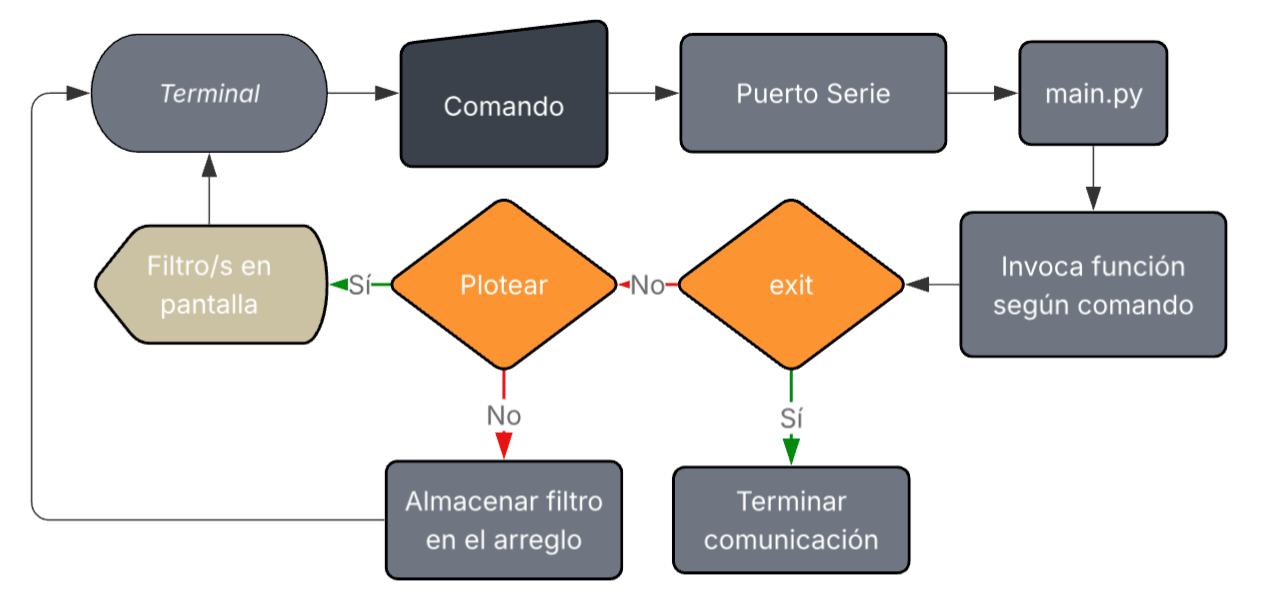
\includegraphics[width=0.9\textwidth]{imagenes/flujo.png}
    \caption{Diagrama de flujo}
    \label{fig:flujo}
\end{figure}
\subsection{Ejemplos de funcionamiento}
Lo que respecta a los ejemplos de funcionamiento, se utilizará un ejemplo por cada tipo de comando
disponible para el usuario.
\subsubsection{Generación de filtros}
    Para el manejo de la creación de filtros mediante el puerto serie, se enviará el siguiente comando
    por la terminal, hacia el puerto serie.
    \begin{terminal}
    generate_filter:0.5,10,10,t
    \end{terminal}
    Donde definimos un filtro con las siguientes características:
    \begin{itemize}
        \item alpha = 0.5
        \item span = 10
        \item sps = 10
        \item rrc = 'True'
    \end{itemize}
    Posteriormente a la primer generación, se generarán 2 filtros más para demostrar el funcionamiento de la herramienta de ploteo.
    \begin{terminal}
    generate_filter:0.9,30,100,t
    generate_filter:0.1,10,5,t
    \end{terminal}
\subsubsection{Ploteo de Filtros en frecuencia}
    Como se explicó anteriormente en este informe, los comandos disponibles para graficar la respuesta al impulso en el dominio de 
    la frecuencia permiten graficar un filtro a la vez o varios en simultáneo. Sabiendo esto, se colocó en la terminal:
    \begin{terminal}
    plot_filter_freq:0
    \end{terminal}
    Como el órden de generación de filtros define el número asociado al mismo, se graficará el filtro 0 en TC.
    \begin{figure}[h]
        \centering
        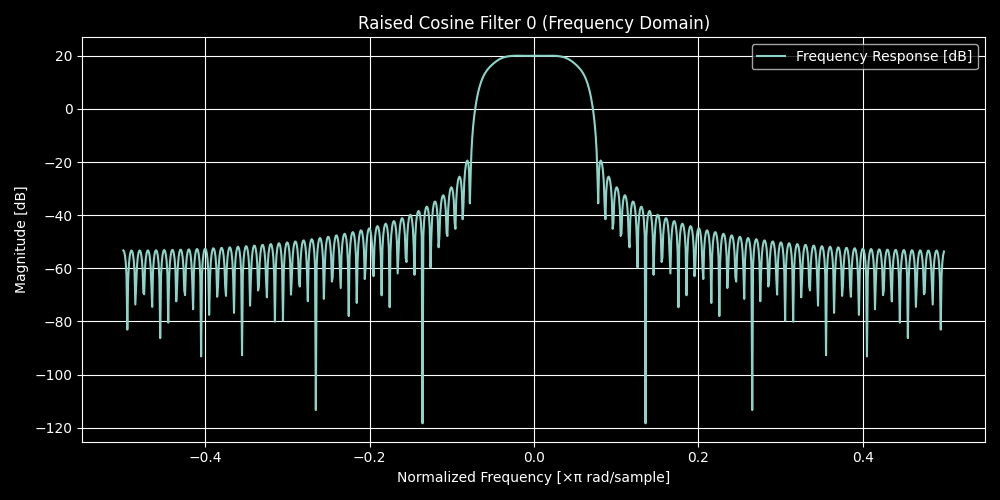
\includegraphics[width=0.9\textwidth]{imagenes/plot_filter_freq.png}
        \caption{Filtro 0 en frecuencia y TC}
        \label{fig:plot_filter_freq}
    \end{figure}
    
    Dada la capacidad del comando, se generará el mismo gráfico pero en TD.
    \begin{terminal}
    plot_filter_freq:0,d
    \end{terminal}
    \begin{figure}[h]
        \centering
        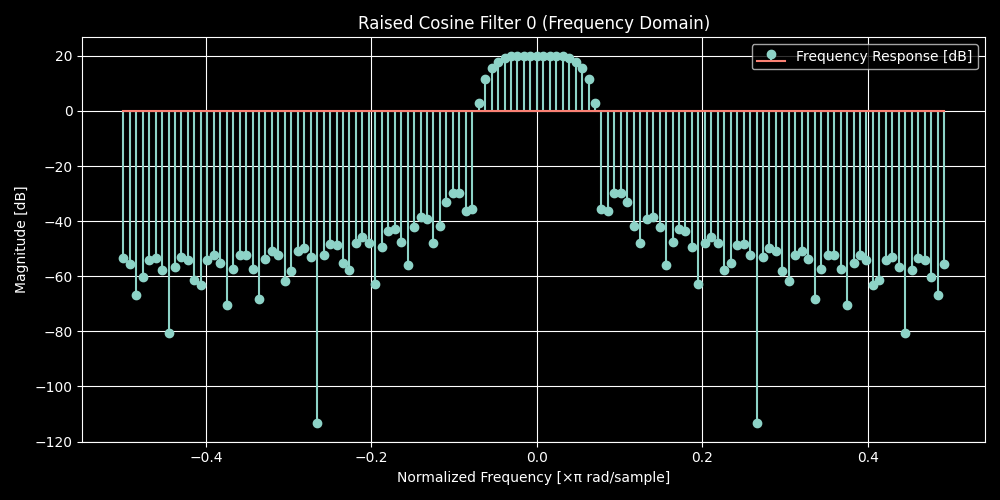
\includegraphics[width=0.9\textwidth]{imagenes/plot_filter_freq_d.png}
        \caption{Filtro 0 en frecuencia y TD}
        \label{fig:plot_filter_freq_d}
    \end{figure}

    Para finalizar con este inciso, se hará uso del comando que permite graficar varios 
    filtros a la vez (Usando tiempo continuo en este caso).
    \begin{terminal}
    plot_all_freq:c
    \end{terminal}
    Donde se obtuvo la siguiente figura.
    \begin{figure}[H]
        \centering
        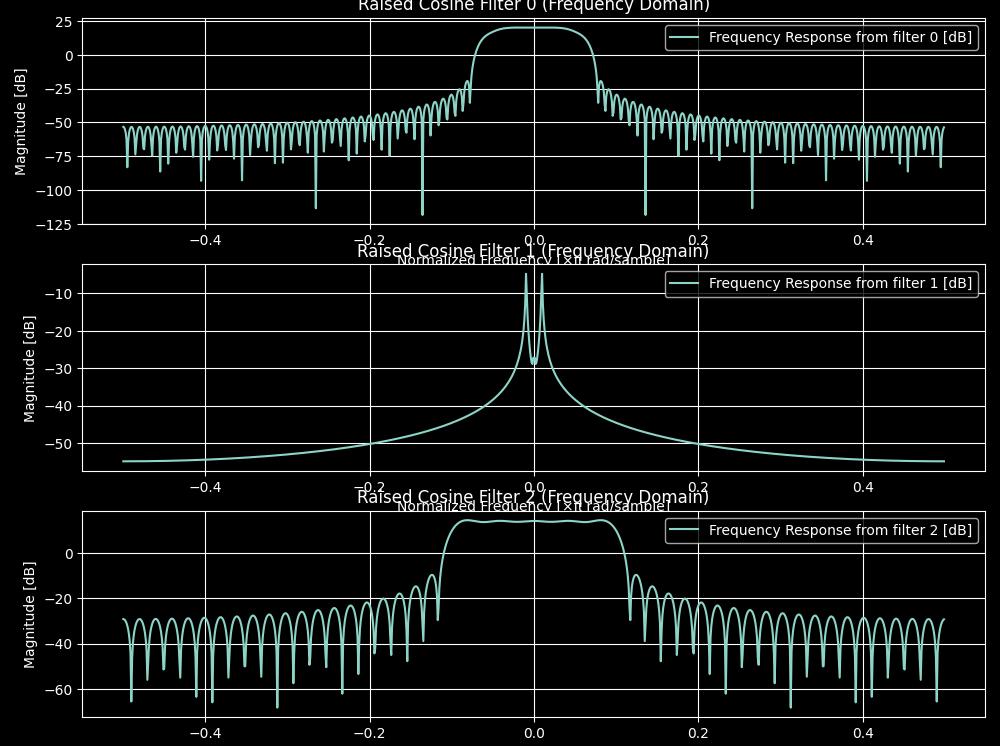
\includegraphics[width=0.9\textwidth]{imagenes/plot_all_freq_c.png}
        \caption{Filtros 0, 1 y 2 en frecuencia y TC.}
        \label{fig:plot_all_freq_c}
    \end{figure}
    Algo clave que se puede observar en la \autoref{fig:plot_all_freq_c} es que, para los filtros
    con un \texttt{alpha} más cercano a 0, la forma del espectro tiende a ser más rectangular, es decir, presenta un ancho de banda mayor.
    Por otra parte, en los filtros con un \texttt{alpha} más cercano a 1 la forma del espectro tiende a ser más suavizada, lo que limita el ancho de banda.
    
    Este fenómeno puede verse con mayor claridad utilizando el siguiente comando.
    \begin{terminal}
    plot_simult_freq:c
    \end{terminal}
    \begin{figure}[H]
        \centering
        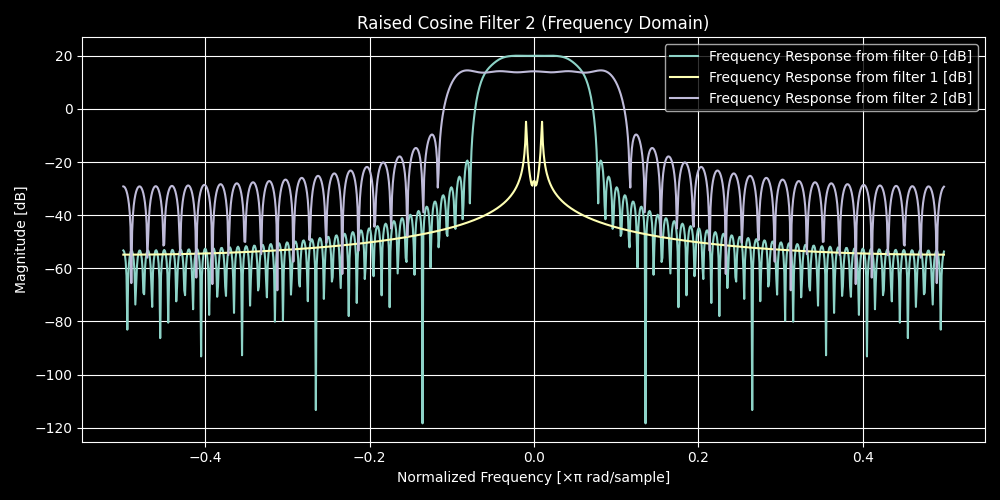
\includegraphics[width=0.9\textwidth]{imagenes/plot_simult_freq.png}
        \caption{Filtros 0, 1 y 2 superpuestos en frecuencia.}
        \label{fig:plot_simult_freq}
    \end{figure}
\subsubsection{Ploteo de Filtros en tiempo}
    Para el dominio temporal, se tienen las mismas funciones que se utilizaron para inciso anterior, con lo cual podemos graficar
    la respuesta al impulso del filtro 0.
    \begin{terminal}
    plot_filter_time:0,c
    \end{terminal}
    \begin{figure}[H]
        \centering
        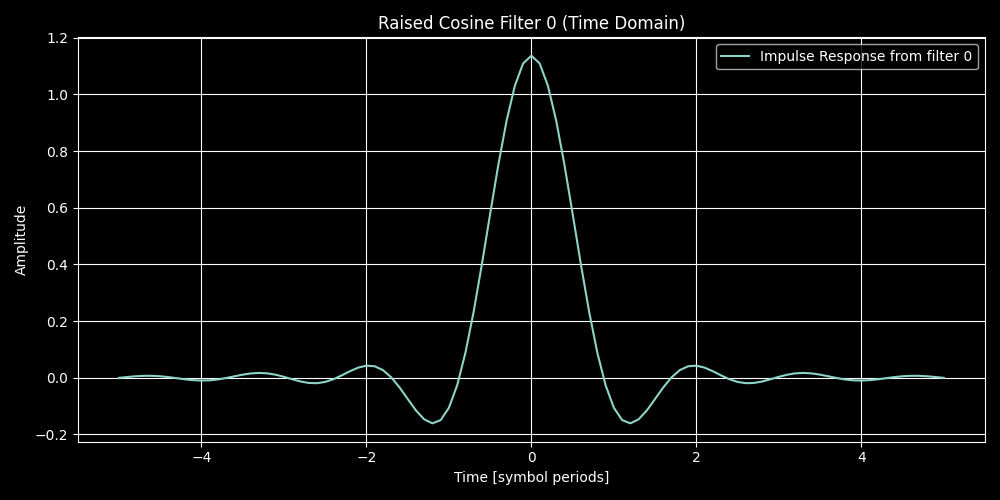
\includegraphics[width=0.9\textwidth]{imagenes/plot_filter_time_c.png}
        \caption{Filtro 0 en el dominio temporal y TC.}
        \label{fig:plot_filter_time_c}
    \end{figure}
    Para un tiempo continuo, se observa la \autoref{fig:plot_filter_time_c}.
    
    De igual manera, se puede realizar para tiempo discreto.
    \begin{terminal}
    plot_filter_time:0,d
    \end{terminal}
    \begin{figure}[H]
        \centering
        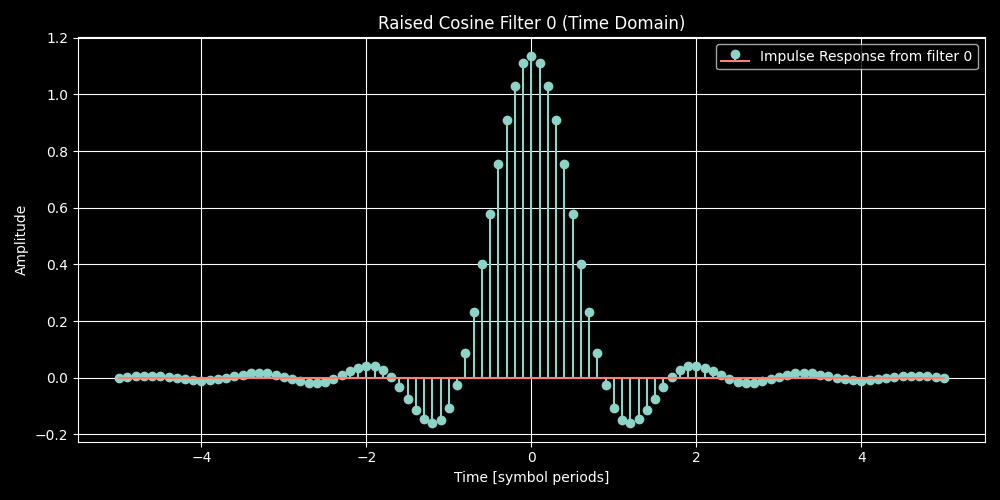
\includegraphics[width=0.9\textwidth]{imagenes/plot_filter_time_d.png}
        \caption{Filtro 0 en el dominio temporal y TD.}
        \label{fig:plot_filter_time_d}
    \end{figure}
    
    Posteriormente, se realizará el ploteo de las respuestas al impulso de todos los filtros en diferentes subplots.
    \begin{terminal}
    plot_all_time:c
    \end{terminal}
    \begin{figure}[H]
        \centering
        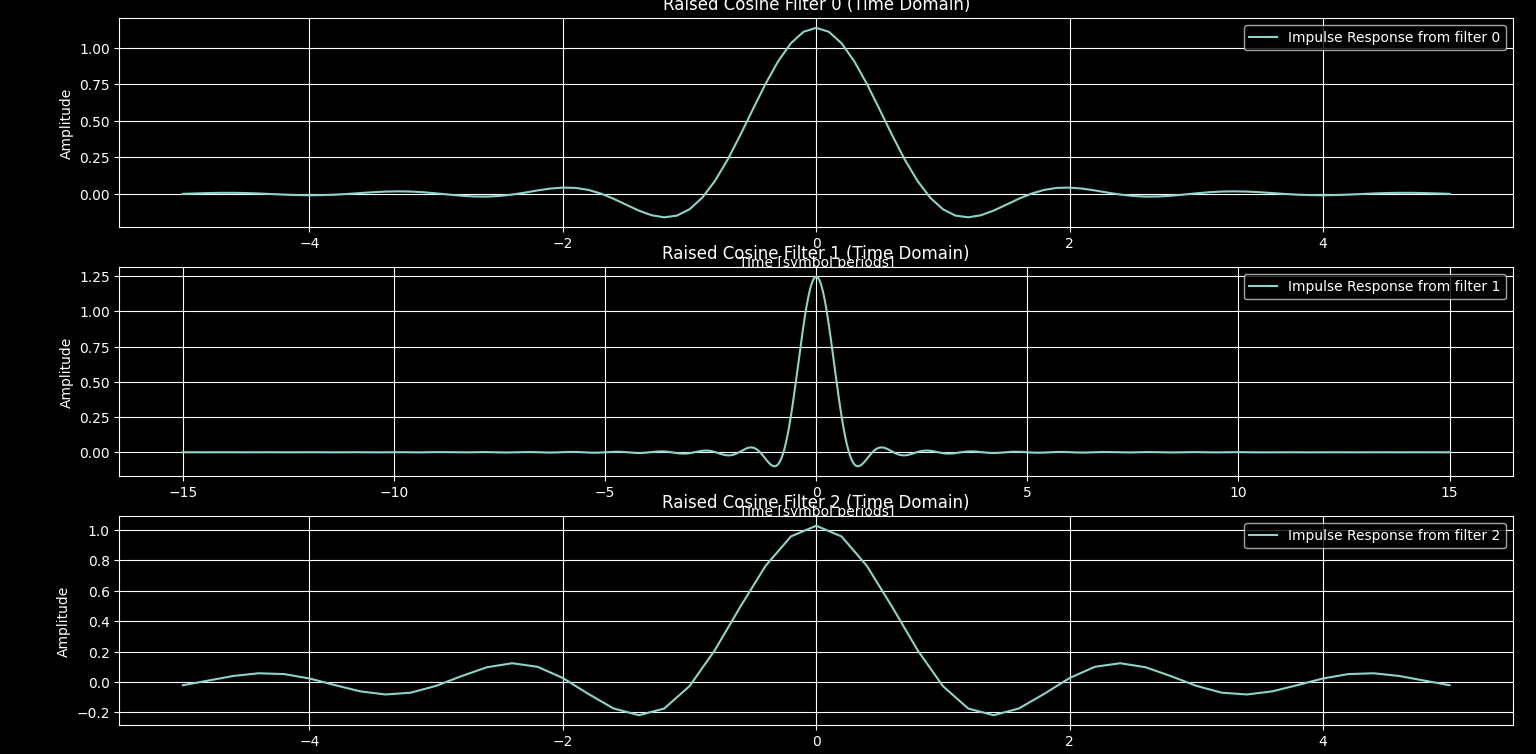
\includegraphics[width=0.9\textwidth]{imagenes/plot_all_time_c.png}
        \caption{Filtros 0, 1 y 2 en el dominio temporal y TC.}
        \label{fig:plot_all_time_c}
    \end{figure}
    Como ya indicaba la frecuencia, para un valor de \texttt{alpha} cercano a 0, se tiene una respuesta
    temporal más suavizada, mientras que para un valor de \texttt{alpha} cercano a 1, la respuesta temporal es mucho mas abrupta.
    
    Por otro lado, en lo que refiere a las muestras por símbolo, la diferencia clara se puede visualizar utilizando el comando
    que nos permite superponer las respuestas.
    \begin{terminal}
    plot_simult_time:c
    \end{terminal}
    Para lo que se obtiene la siguiente figura.
    \begin{figure}[H]
        \centering
        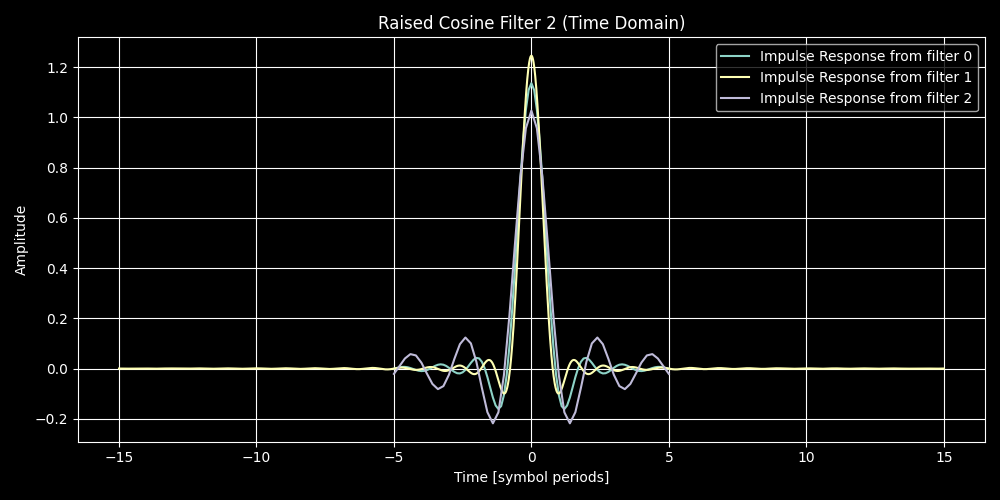
\includegraphics[width=0.9\textwidth]{imagenes/plot_simult_time.png}
        \caption{Filtros 0, 1 y 2 superpuestos en tiempo.}
        \label{fig:plot_simult_time}
    \end{figure}
    Donde se ve claramente que, para un valor de muestras por símbolo mayor, la curva se representa de una manera mucho más suavizada
    y representativa de lo que sería una respuesta de un sistema real.
\subsubsection{Ploteo Total}
    En caso de querer visualizar las respuestas al impulso y la respuesta en frecuencia de todos los
    filtros utilizados como ejemplo, se puede utilizar el siguiente comando.
    \begin{terminal}
    plot_simult_all:c
    \end{terminal}
    Donde se generará la gráfica que muestre el apartado en frecuencia y en tiempo de todos los filtros
    superpuestos entre sí, como se ve a continuación.
    \begin{figure}[H]
        \centering
        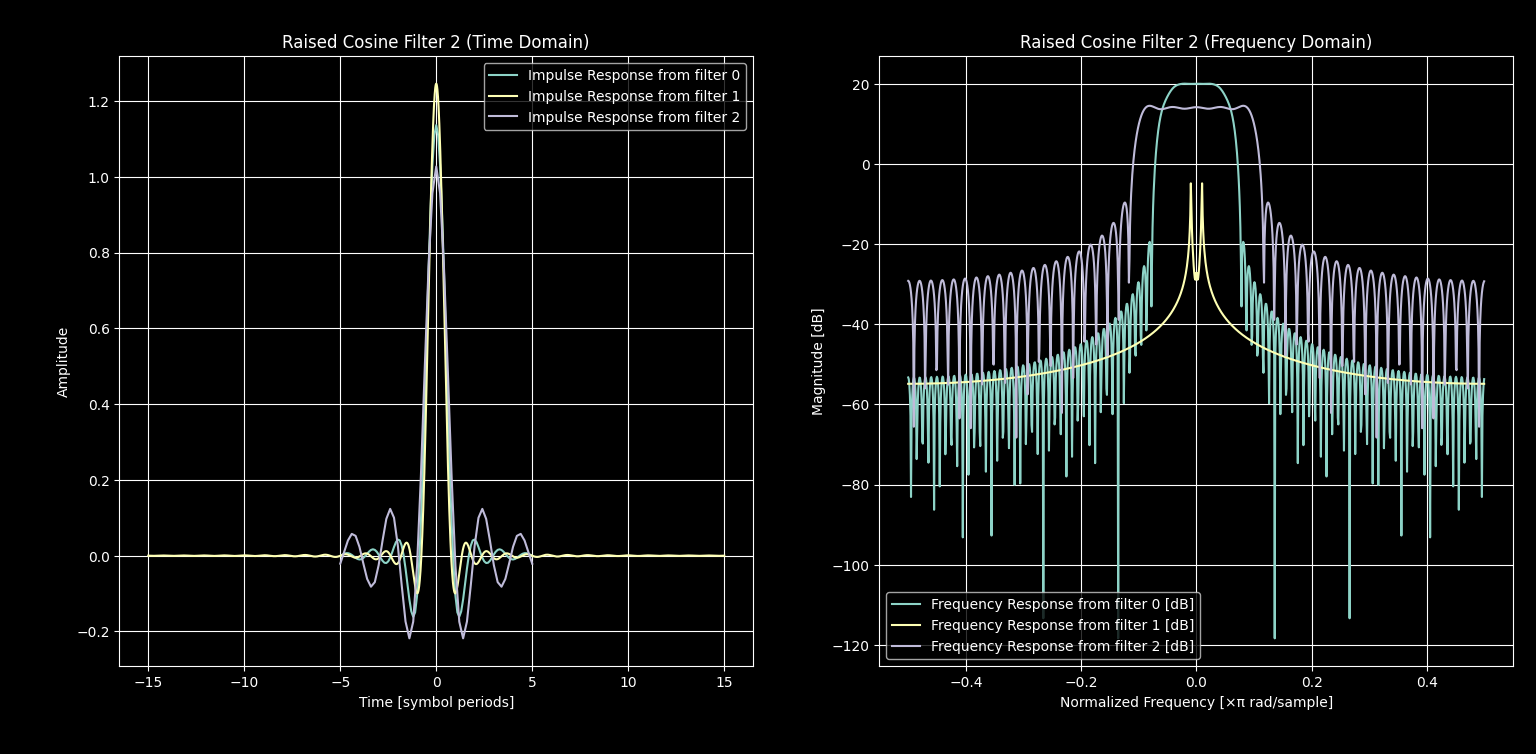
\includegraphics[width=0.9\textwidth]{imagenes/plot_simult_all.png}
        \caption{Filtros 0, 1 y 2 superpuestos en tiempo y frecuencia.}
        \label{fig:plot_simult_all}
    \end{figure}
\subsubsection{RC vs. RRC}
    Finalizando con la parte de análisis, se generarán dos filtros muy parecidos, pero con una diferencia; Uno será 
    un filtro Raised Cosine y el otro será un filtro Root Raised Cosine.
    
    El objetivo de este experimento es visualizar de manera clara las diferencias
    entre un tipo de filtro y otro para un caso en el que ambos presentan los mismos parámetros.
    
    Se colocará por la terminal los siguientes comandos.
    \begin{terminal}
    generate_filter:0.5,10,10,t
    generate_filter:0.5,10,10,f
    plot_simult_all:c
    \end{terminal}
    Entonces, se generó:
    \begin{itemize}
        \item \textbf{Filtro 0}:(\texttt{alpha}=0.5,\texttt{span}=10,\texttt{sps}=10,\texttt{RRC}=True)
        \item \textbf{Filtro 1}:(\texttt{alpha}=0.5,\texttt{span}=10,\texttt{sps}=10,\texttt{RRC}=False)
        \item \textbf{Plot simultáneo de tiempo y frecuencia}
    \end{itemize}
    \begin{figure}[H]
        \centering
        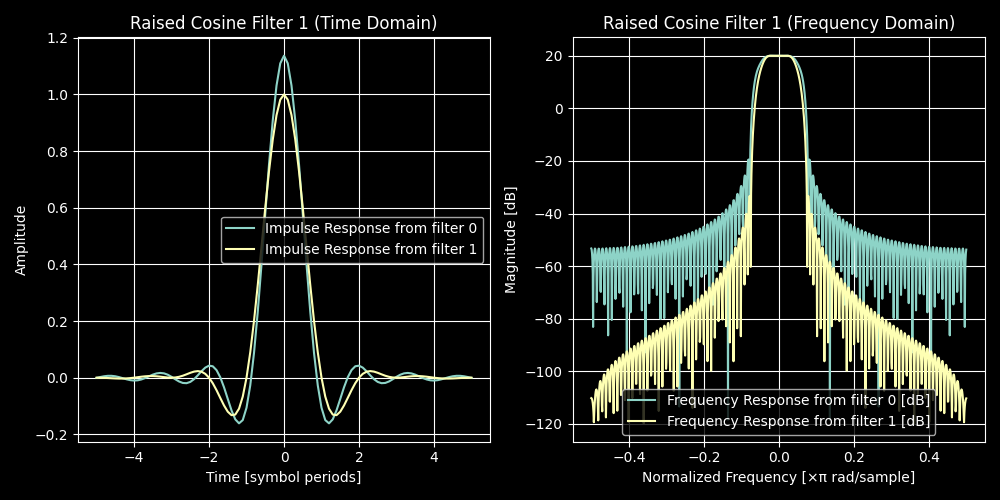
\includegraphics[width=0.9\textwidth]{imagenes/plot_simult_all_RCyRRC.png}
        \caption{Filtros RC y RRC superpuestos en tiempo y frecuencia.}
        \label{fig:plot_simult_all_RCyRRC}
    \end{figure}
    Se confeccionó una tabla comparativa para ver los resultados.
    \begin{table}[H]
        \centering
        \begin{tabular}{|l | c | c|}   % l=izquierda, c=centrado, r=derecha
            \hline
            \textbf{Dominio} & \textbf{Filtro RC} & \textbf{Filtro RRC} \\
            \hline
            Tiempo         & Ceros en $k*T$         &  No hay ceros en $k*T$            \\
            \hline
            Frecuencia     & Ajuste de cero ISI     &  Pérdidas en bandas no útiles     \\
            \hline
        \end{tabular}
        \caption{Comparación de tipos de filtro}
        \label{tab:comparacion}
    \end{table}
    El apartado más significativo fue el de la frecuencia, donde se puede ver perfectamente el efecto de la ISI nula.
    A medida que se aleja la frecuencia de la banda central, se atenuan las pérdidas en las bandas no deseadas.

\newpage

\section{Conclusión}
Se cierra este informe concluyendo que, en lo que respecta a \textbf{Python},
la capacidad del lenguaje para el manejo de datos es extremadamente útil. Las posibilidades que nos permiten
los scripts es ilimitada en el área del procesamiento de información, lo cuál será de gran ayuda en caso de utilizar
la comunicación en serie para laboratorios posteriores.

La dificultad principal fue adaptar correctamente la comunicación serial con el script principal, 
debido a malinterpretaciones de la consigna, lo cual se solucionó modificando el script para que en vez de que se haga en bucle, 
se invoque al declararse como función.
\end{document}
